\begin{frame}{Measuring the top-quark properties is key to test the validity of the SM. The LHC is a top-quark factory.}
\centering
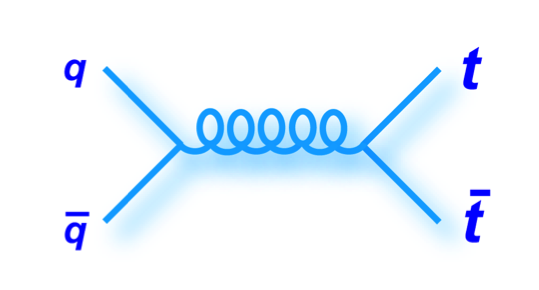
\includegraphics[height=0.25\textheight]{./plots/ttbar_1.png}
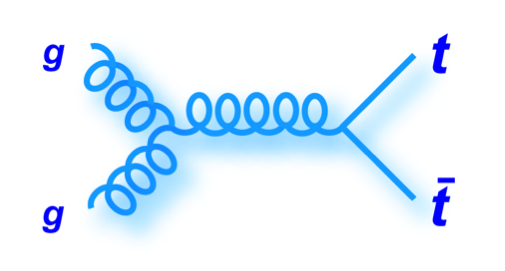
\includegraphics[height=0.25\textheight]{./plots/ttbar_2.png}
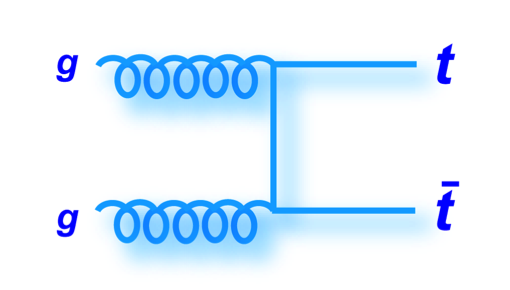
\includegraphics[height=0.25\textheight]{./plots/ttbar_3.png}
\begin{enumerate}
\item[o] The top quark is the heaviest elementary particle $\rightarrow$ largest Yukawa coupling.
\end{enumerate}
\centering
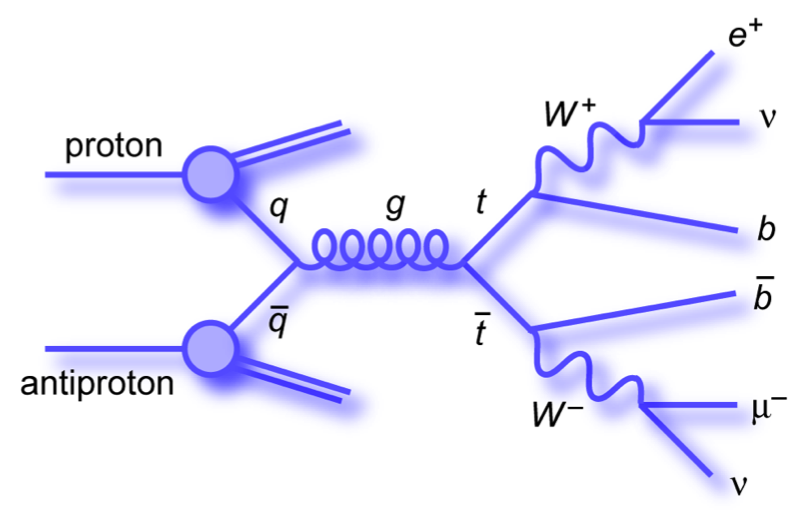
\includegraphics[height=0.3\textheight]{./plots/ttbar_4.png}
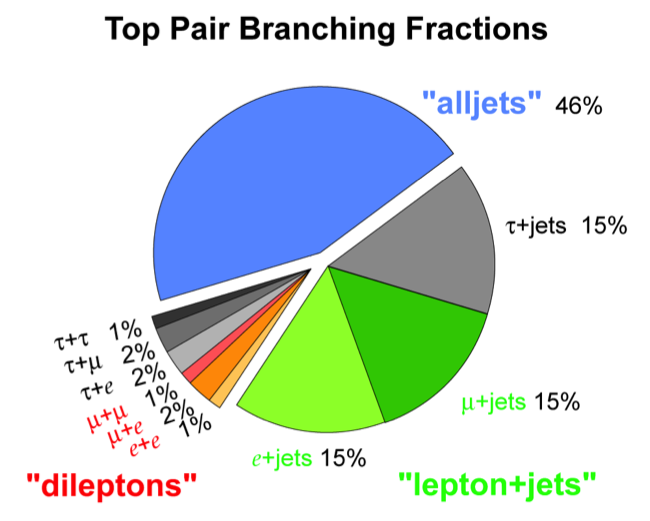
\includegraphics[height=0.3\textheight]{./plots/ttbar_5.png}
\begin{enumerate}
\item[o] Our analysis is top-quark pair-production in $e-\mu$ (2\% of ttbar).
\end{enumerate}
\end{frame}
\clearpage


\begin{frame} {Theoretical simulation vs. experimental analysis}
\begin{enumerate}
\item[o] Theoretical simulation: generated (truth) are known $\rightarrow$ observed (reco).
\item[o] Experimental analysis: observed (reco) are known $\rightarrow$ truth (nature)
\end{enumerate}
\centering
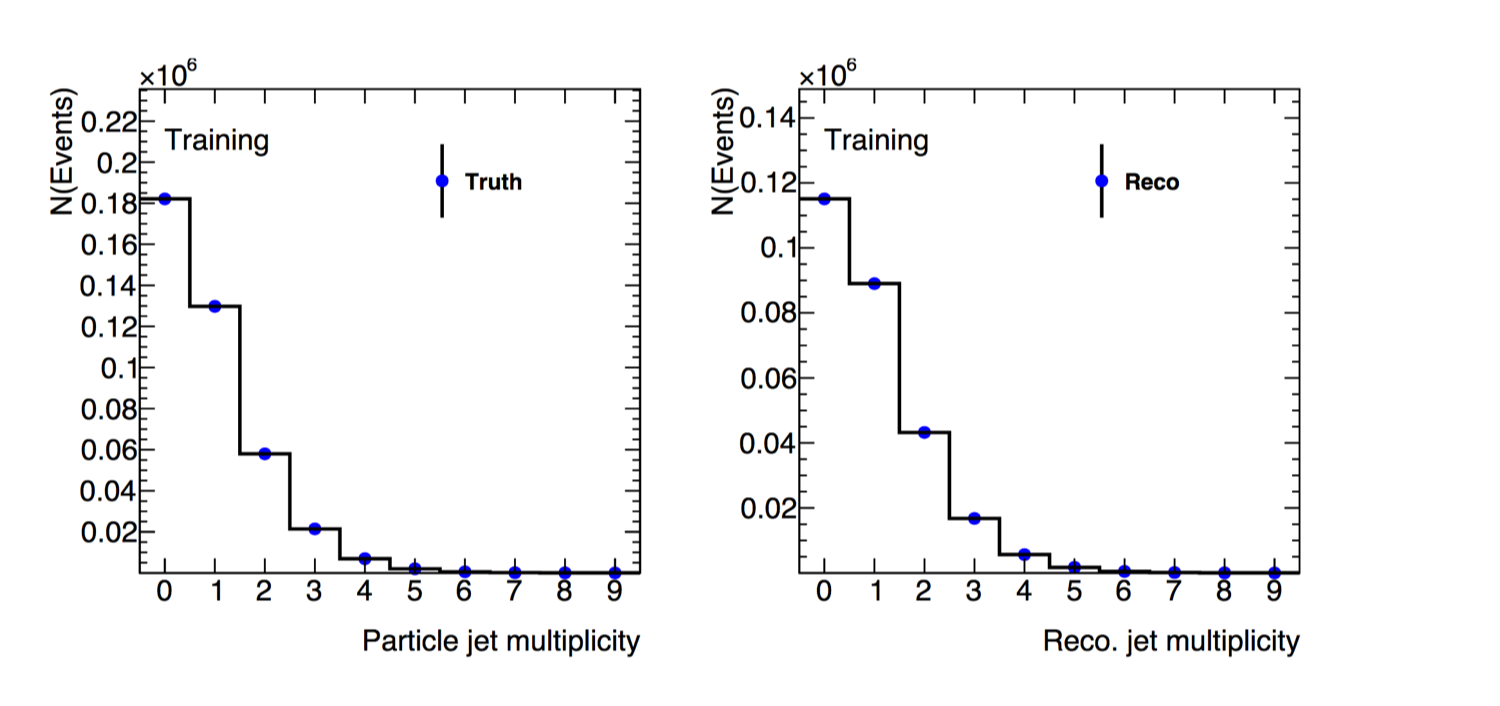
\includegraphics[height=0.5\textheight]{./plots/jet_multiplicity.png}
\begin{enumerate}
\item[o] The shapes of the distributions of the truth and reco observables for the training of the unfolding are very similar, but not identical (especially in the first bins). 
\end{enumerate}
\end{frame}
\clearpage


\begin{frame} {The 2D histogram of the migration matrix}
\begin{enumerate}
\item[o] The migration matrix between truth and reco is used in the traditional unfolding.
\item[o] Unfolding = inferring the generated (truth) from the observed (reconstructed).
\end{enumerate}
\centering
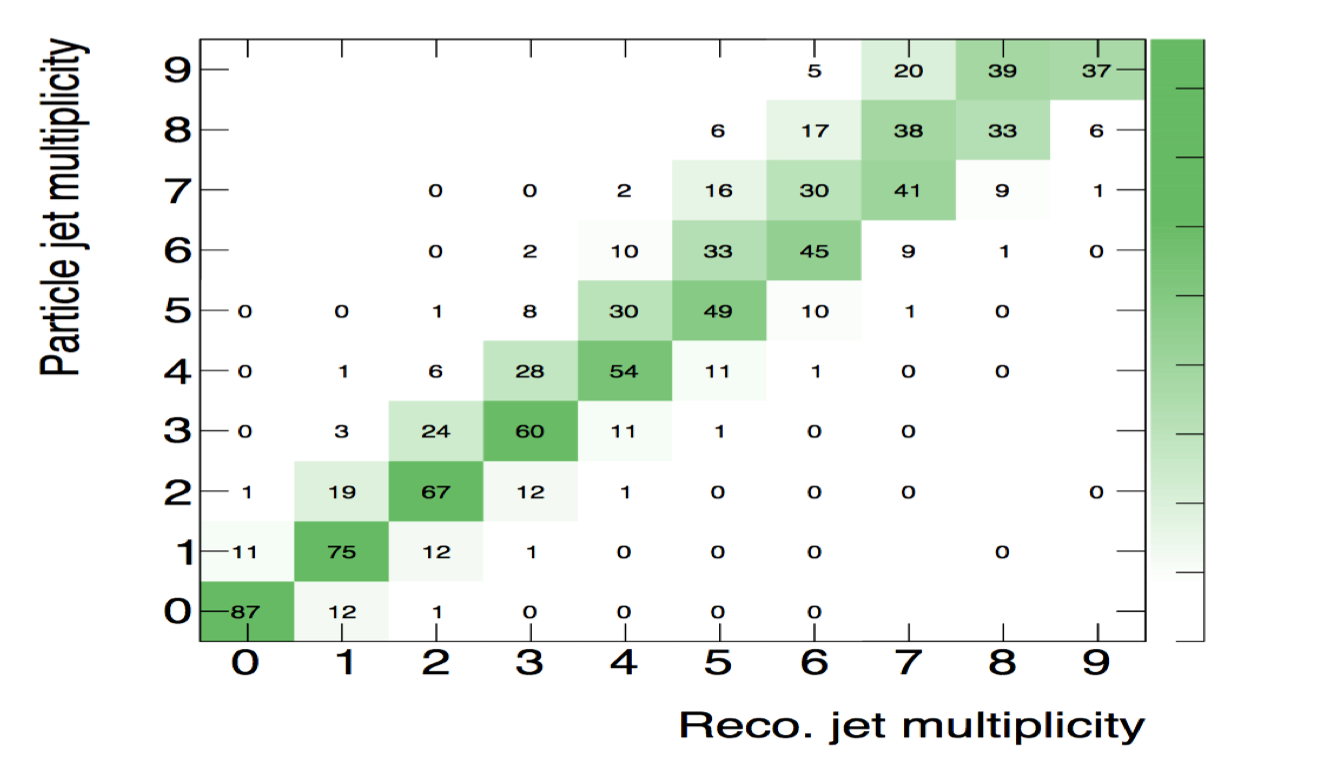
\includegraphics[height=0.5\textheight]{./plots/jet_multiplicity_migration_matrix.png}
\begin{enumerate}
\item[o] The more diagonalizable matrix, the easier unfolding will be.
\item[o] Events are migrating from one truth bin to other bins for reco, and vice-versa.
\end{enumerate}
\end{frame}
\clearpage


\begin{frame}{A new approach: use machine learning to \emph{learn} how to unfold observed (reco) to true (generated).}
\begin{enumerate}
\item[o] \href{https://arxiv.org/pdf/1712.01814.pdf}{arXiv:1712:01814}
\end{enumerate}
\centering
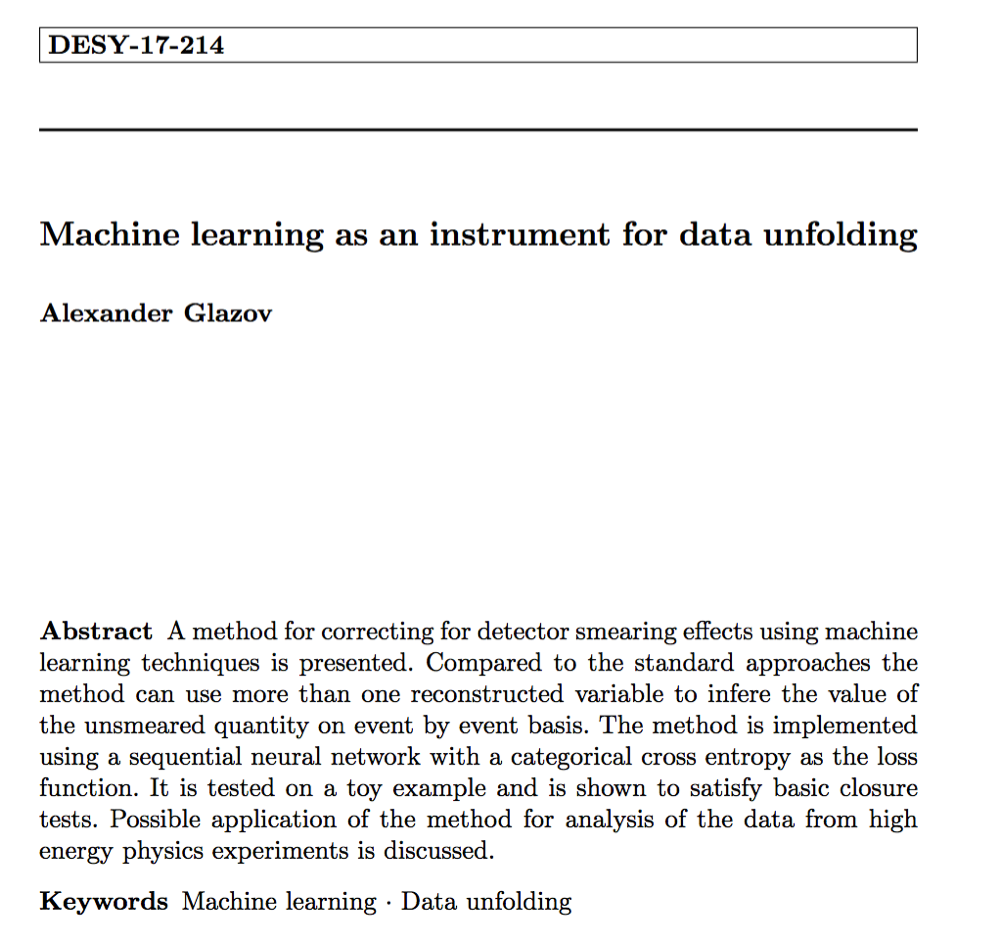
\includegraphics[height=0.7\textheight]{./plots/PaperToyData.png}
\end{frame}
\clearpage

\begin{frame}{Two unfolding methods: traditional and ML.}
\begin{enumerate}
\item[o] Traditional: binned migration matrix with only one variable.
\item[o] Machine learning: a continuous function of several variables.
\end{enumerate}
\centering
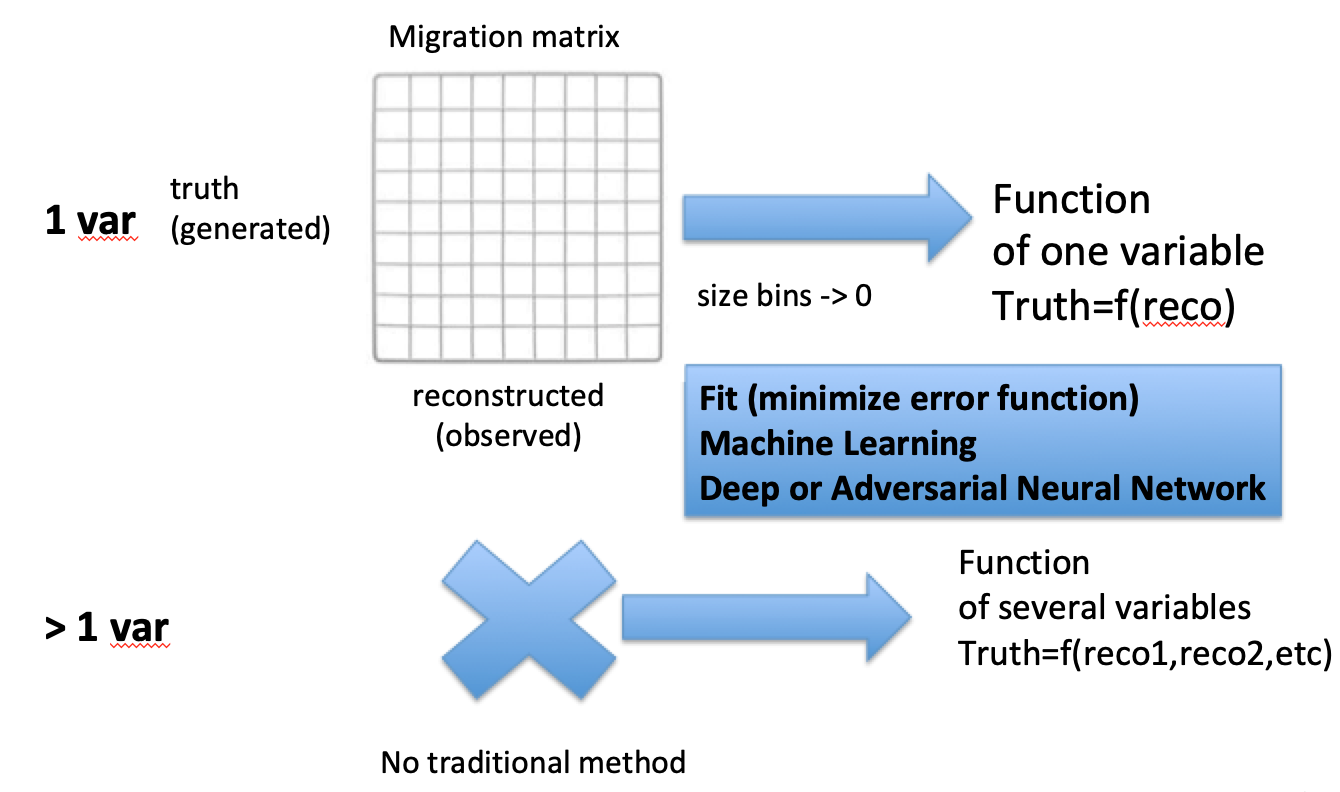
\includegraphics[height=0.70\textheight]{./plots/Unfolding_Traditional_ML.png}
\end{frame}
\clearpage



\begin{frame}{Physics problem: index of truth jet pt = f (reco jet pt) = ?}
\centering
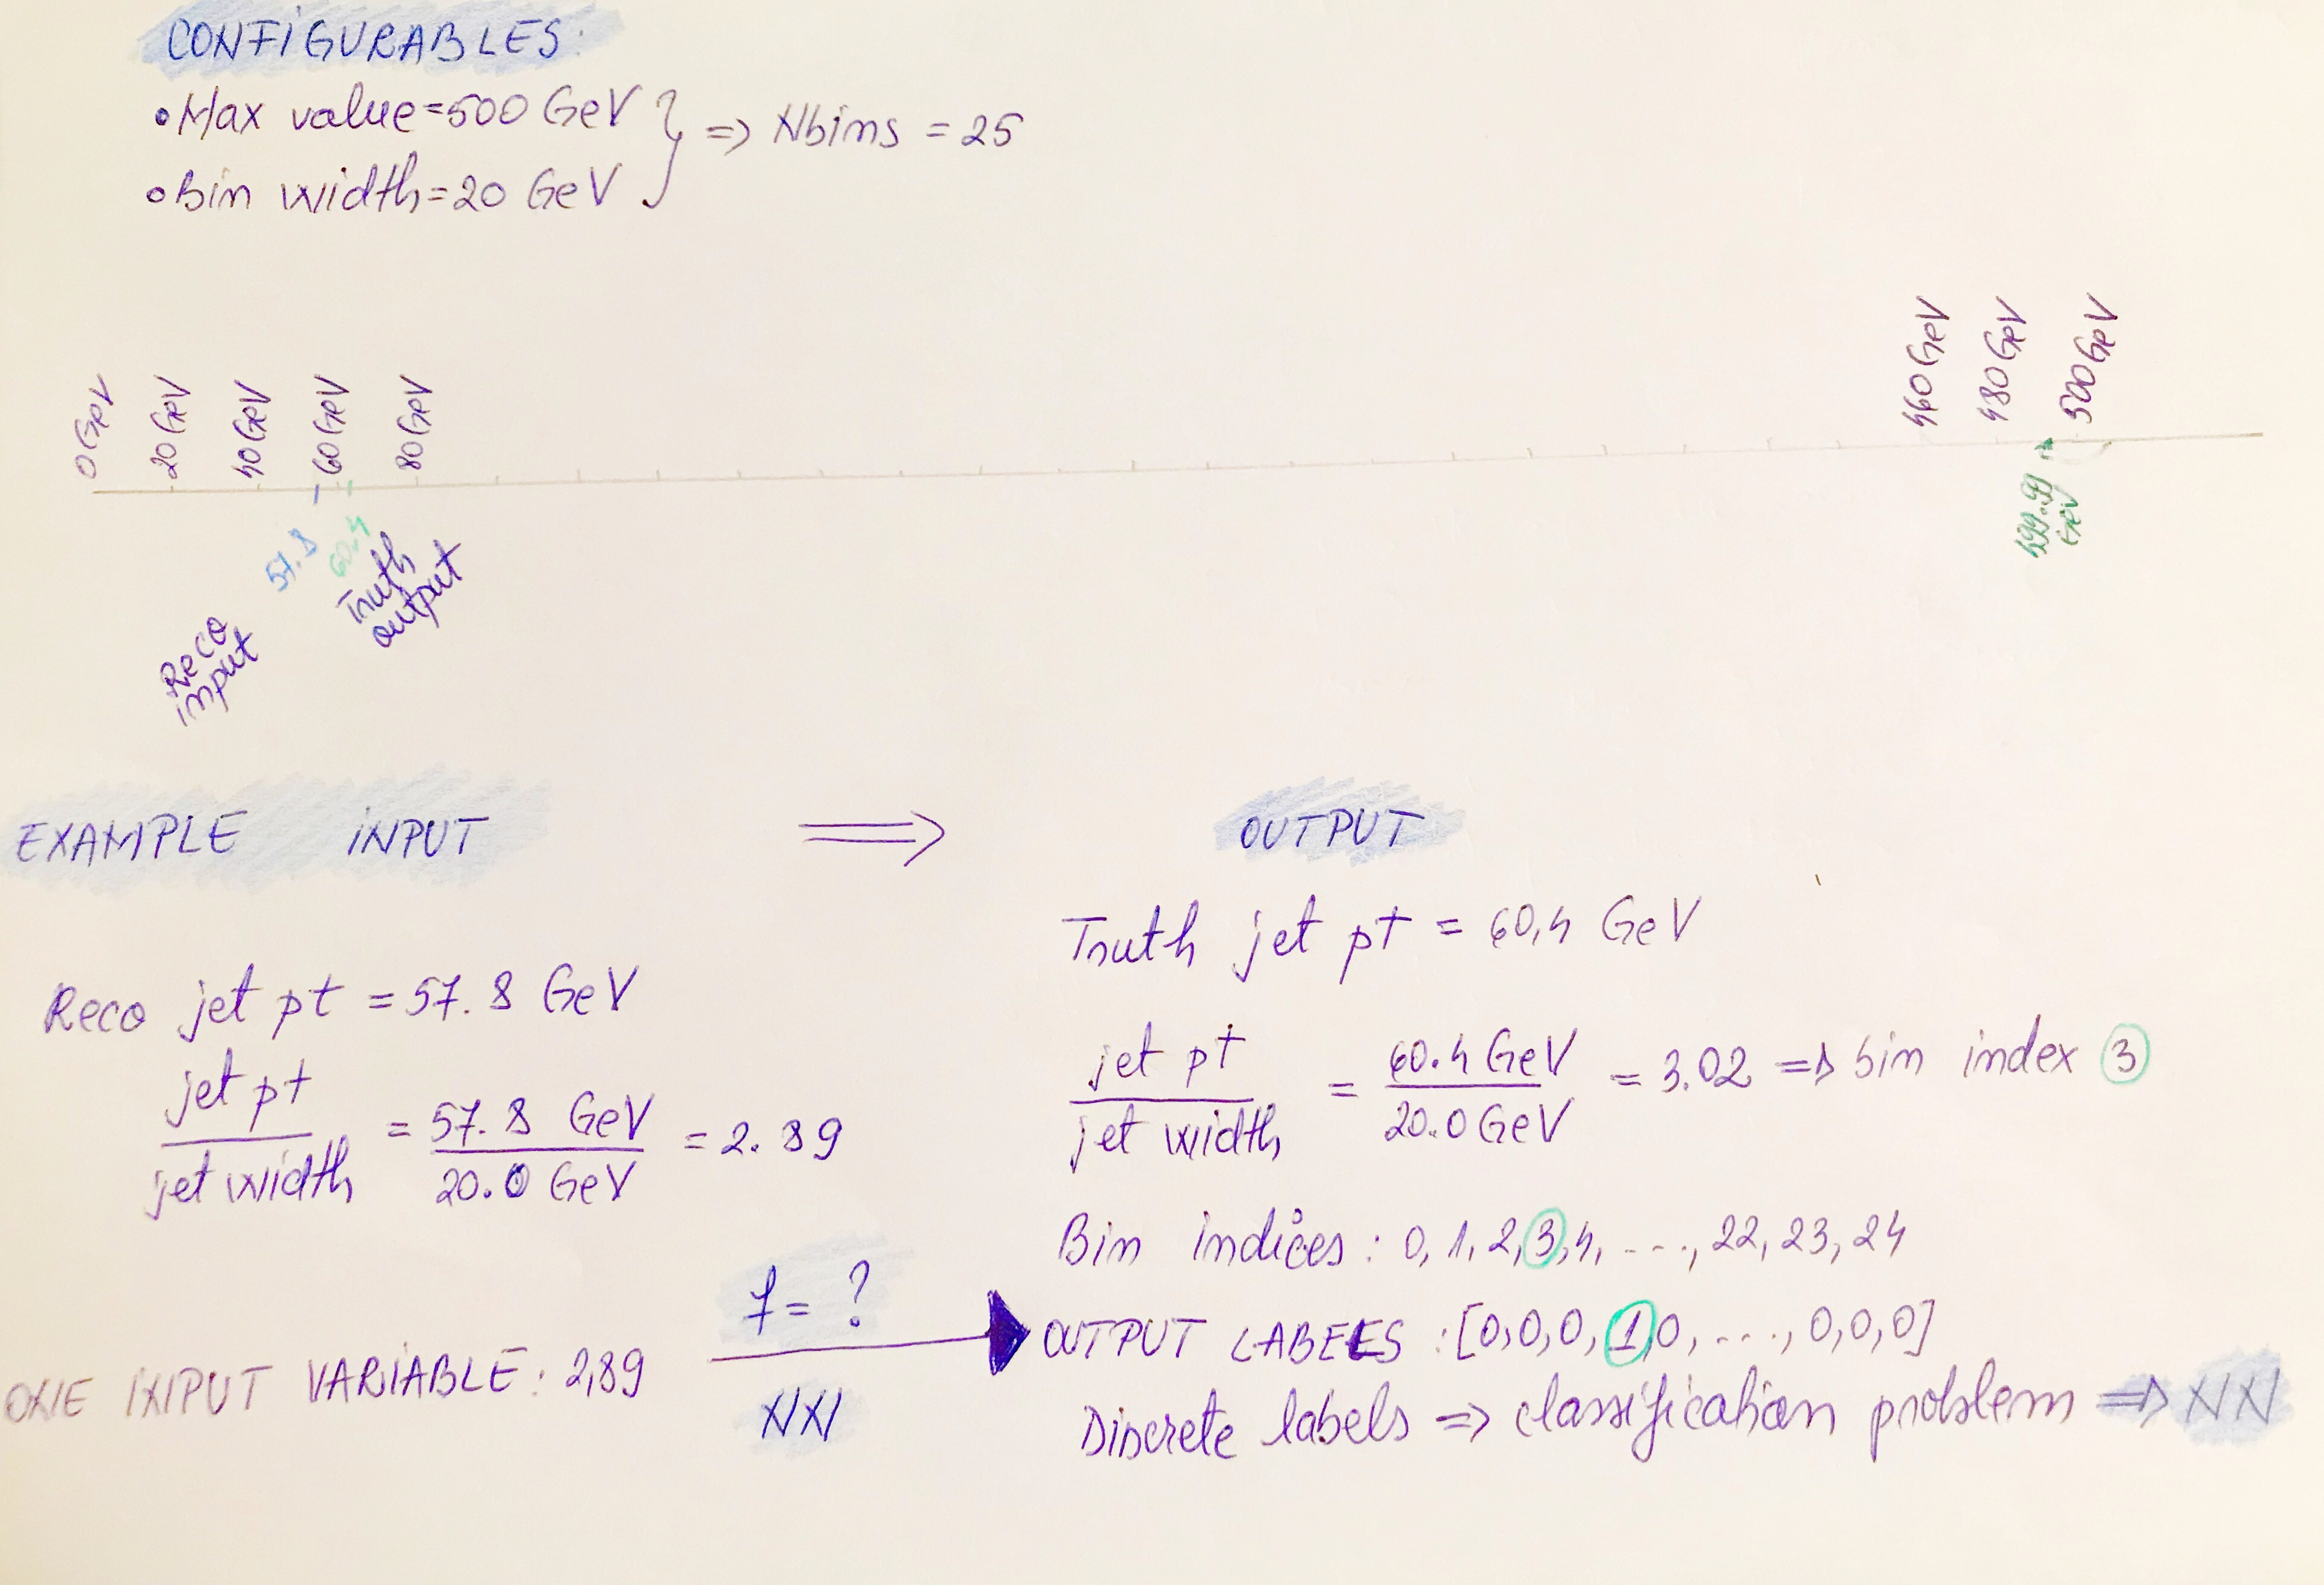
\includegraphics[height=0.80\textheight]{./plots/PhysicsProblem.jpg}
\end{frame}
\clearpage

\begin{frame}{The solution is using these NN architectures.}
\centering
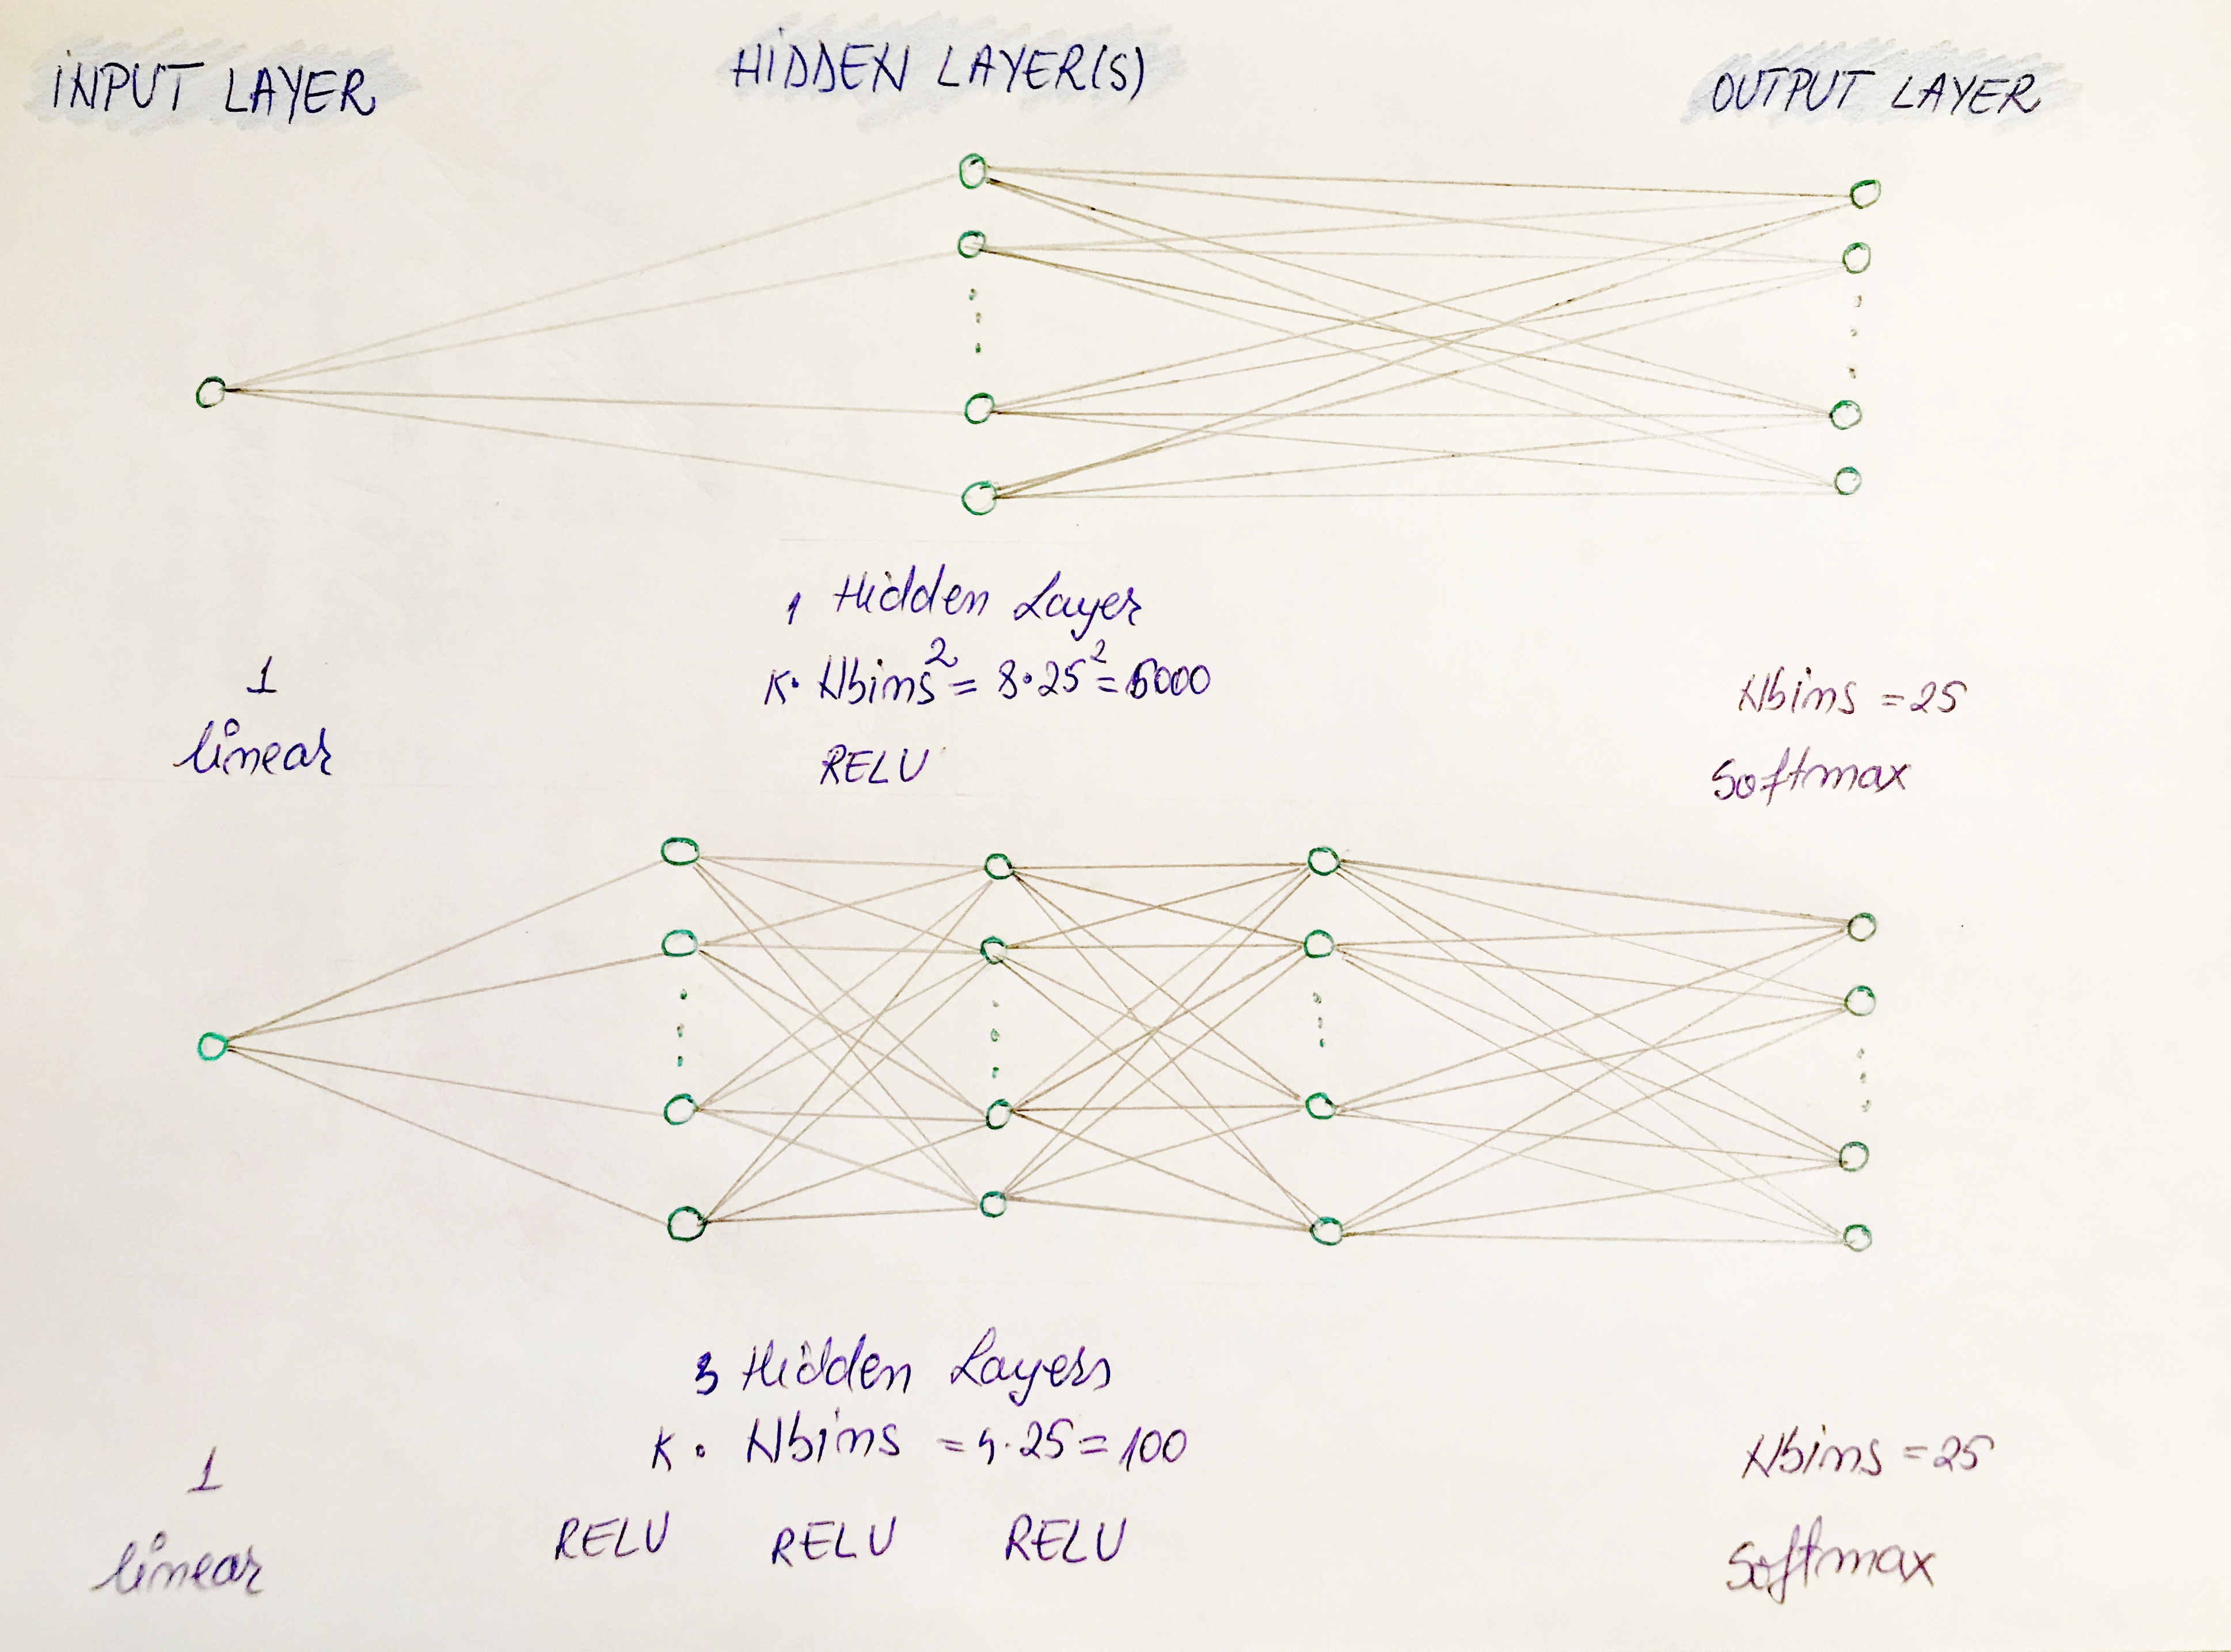
\includegraphics[height=0.80\textheight]{./plots/NNArchitecture.jpg}
\end{frame}
\clearpage

\begin{frame}{The NN is implemented in TensorFlow, via Keras, in Python.}
\centering

\includegraphics[height=0.25\textheight]{./plots/TensorFlow_Keras.png}

\includegraphics[height=0.25\textheight]{./plots/Python.png}
\begin{enumerate}
\item[o] Ran the DNN software for unfolding by DESY Hamburg.
\item[o] Ran on lxplus using the ML software docker image via singularity.
\item[o] Read the ROOT file via the uproot package.
\item[o] Trained  the NNs in Python using Keras and TensorFlow.
\end{enumerate}
\ \\
\ \\
\begin{enumerate}
\item[o] Fine tuned the NN hyper parameters for our ROOT data sample.
\item[o] One NN training is the first step of the iterative unfolding procedure. 
\end{enumerate}
\end{frame}
\clearpage

\begin{frame}{Summary and Next Steps}
\begin{enumerate}
\item[o] Studied Unfolding of the jet pt distributions in ttbar e-mu analysis.
\item[o] Bin of truth jet pt = f (reco jet pt) = ?
\item[o] Discrete output values  $\rightarrow$ classification problem $\rightarrow$ NN.
\item[o] Coded using Tensor Flow via Keras in Python.
\item[o] Followed code example with toy data in arXiv (\href{https://arxiv.org/pdf/1712.01814.pdf}{link for arXiv:1712:01814}).
\item[o] Fine tuned NN hyper-parameters and architecture for our jet data.
\item[o] The chosen NN outperforms the one from the toy data.
\item[o] The project code and report are in GitLab (\href{https://gitlab.cern.ch/lciucu/MLUnfolding/}{link}).
\end{enumerate}
\ \\
\ \\
\begin{enumerate}
\item[o] Training recursively several NNs of the found architecture.
\begin{enumerate}
\item[o] One NN training is just the first (zeroth) step in the NN unfolding method.
\end{enumerate}
\item[o] Use more data (more events and leading jets).
\item[o] Add other input variables (e.g. jet eta).
\end{enumerate}
\end{frame}
\clearpage
